This section will discuss the components of our SyVOLT prover tool. In particular, the first section will focus on a high-level discussion of how transformations and contracts are consumed into the prover, the proving process, and what information is presented back to the user. The second section takes a deeper look into each of these components, focusing on the essential technologies.

\subsection{Tool Overview}
This section will briefly touch on the steps for how a contract is proved on a DSLTrans transformation using our contract proving tool.


\subsubsection{Generation of the Transformation and Contracts}
The starting point for our tool is the building of the DSLTrans transformation and contracts.

Previous research activities at the Modelling, Simulation and Design Lab at McGill University led to the creation of \textbf{AToM$^3$}~\cite{atom3:2002}. This visual editor allowed us to create DSLTrans transformations and contracts visually.

These principles were then used to build a plugin for the Eclipse development environment CITE. This allows our prover to be integrated with the rich ecosystem of Eclipse. An example of a transformation within the Eclipse plugin is seen in Figure~\ref{fig:eclipse_frontend}.

\begin{figure}
\centering
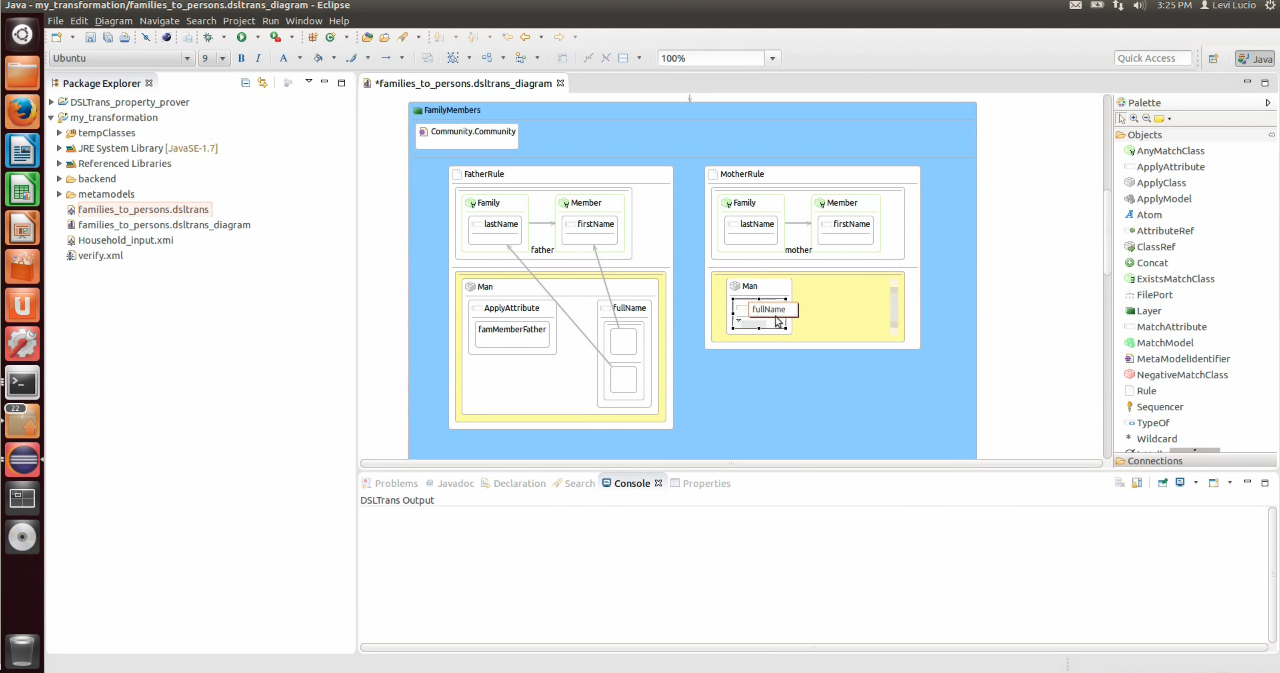
\includegraphics[width=0.45\textwidth]{figures/syvolt_prover/eclipse_frontend}
\caption{The transformation editor within Eclipse}
\label{fig:eclipse_frontend}
\end{figure}

We have also developed a plugin for the MPS editor. This provides us with a number of desirable features, such as deep integration into the tool, such as auto-completion and error checking. ADD FIGURE HERE

Declarative ATL transformations can also be converted into DSLTrans transformations using a higher-order transformation we have developed~\cite{Oakes2016}. Our results show that these automatically-produced transformations are equivalent to hand-built versions.

%
%\markus{The first part of this subsection really isn't related to what the
%subsection heading says. Maybe move this stuff above the subsection?} SyVOLT
%proves that pre-/post-condition contracts hold for a model transformation. Such
%contracts establish relations between patterns occurring in input and output
%models of a model transformation. If a contract holds, then a formal guarantee
%exists that whenever an input model contains the pattern specified in the
%pre-condition of the contract, the output model contains the pattern specified
%in the post-condition part of the contract and any traceability relations
%between the two\markus{The part after ``and'' does not work grammatically.}.
%Due to the graph-like structure of the pre and post conditions of contracts, the
%visual representation of the contract in SyVolt editor allows the user to
%quickly build and intuitively understand their meaning\markus{Only true to a
%degree. The string concatenation syntax, for example, is really bad!}.
%If a textual (logical or mathematical) editor where to be used, the user would
%need an extra system of identifiers to correctly prescribe the associations
%between pre and post-condition elements whereas in the visual representation,
%the user graphically builds the associations between those elements\markus{That
%part is certainly true. The story for he strings is different, though :-)}.
%\levi{Claudio, I don't understand this sentence}
%\cgg{Please tell me now if you can understand it.}
%\markus{Looking at the other subsections here, I think this one really should
%not be emphasized by being the first. Maybe having a subsection ``tool
%support'' at the end? There you could also put the ATL stuff which I think is
%out of place here; see below.}
%
%The visual representation of a contract has all the necessary information to
%derive the correct logical expression to be used by the internal SyVolt prover.


\subsubsection{Generation of Proving Artifacts}

The contract prover requires a number of concrete artifacts in order to prove the contract over all executions of the transformation. More information on the tooling can be found below. However, we wish to emphasize that the prover is able to generate all necessary artifacts directly from the transformation and contracts. No further user input is required beyond the starting of the proving process.

%The
%proving process is fully automatic and the all formal details are completely
%hidded from the user, who only needs to specify a set of contracts for the
%transformation being verified. Once the transformation and the contracts of
%interest are created, one command will start the property proving process. This
%process will automatically create all required artifacts (as detailed in the
%following section), run the process, and then provide the results to the user
%within the Eclipse environment, as seen in Figure~\ref{fig:output}. This allows
%the user to continually stay within the Eclipse environment, which is where he
%develops the contracts and the model transformations.
%\markus{Hmmm. Is it really about staying withing Eclipse? I think that, while
%this is useful, the more important point is that the user stays on the
%abstraction level of the contracts and properties, and is not exposed to low
%level prover stuff.}



\subsubsection{Symbolic Execution Process}

As discussed in Section~\ref{sec:contract_proving}, our symbolic execution process will generate all path conditions which represent the infinite set of all possible transformation executions.

The contracts are then proved on these path conditions. Output as seen in Figure~\ref{fig:output} is then presented to the user as the result of the proof.


\begin{figure}
\centering
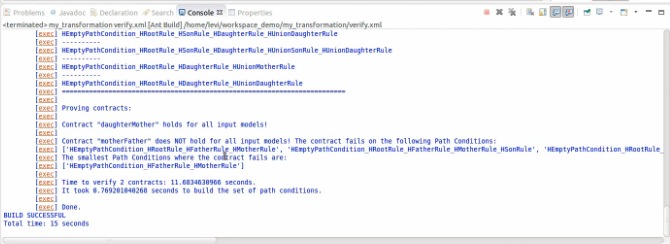
\includegraphics[width=0.45\textwidth]{figures/syvolt_prover/output}
\caption{The results of the contract prover}
\label{fig:output}
\end{figure}

Our technique is exhaustive, in the sense that whenever a contract holds, it
will hold for \emph{all} possible input models of a transformation. This is
possible because SyVOLT operates on specifications of outplace\markus{Is this a
word :-) ?} model transformations where unbounded loops and model element
deletions are not allowed. SyVOLT thus proves contracts in an input-independent
manner, relying only on the specification of the transformation itself. The
soundness and completeness of our technique is described in~\cite{Lucio2014}.


%Our technique shares its principles\markus{What does this mean? Is it symbolic
%Ex or not? If not, what exactly does it share and how is it different?} with
%symbolic execution, a well-established code verification method.
%The underlying idea entails building a finite representation of the (infinite)
%set of model transformation computations, such that properties of interest can
%be proved\markus{Check at the end: do we use proved and proven consistently?} on
%such finite representation and extrapolated\markus{Sounds like this is not
%safe. Use another word?} to the originally infinite set of possible
%computations.
%
%Our model transformation verification technique relies on typed graphs as the
%means to internally represent both symbolic executions and contracts. SyVOLT
%then reasons over these graphs to build a proof that contracts hold or do not
%hold. Note that by using a typed graph representation, our technique can prove
%contracts that include constraints on the attributes of the input and output
%models. 
%
%\levi{keep the text from here on?}\markus{If we use an example here, we should
%also use one in the preceding sections. Otherwise remove.} An example of this
%would be in the Families-To-Persons transformation from the ATL zoo [CITE]. In
%this transformation, the name for a person in the output graph is a
%concatenation of two strings \cgg{instead of ''strings``, should be
%''attributes``}\markus{string values in attributes?} from elements in the input
%graph. Our contract prover can prove that this concatenation will be valid in
%all cases.
%


\subsection{Tool Technologies}


The guiding principle of the Modelling, Design, and Simulation Lab of McGill University, where this research was developed, is that all tools and processes be
explicitly modelled at an appropriate abstraction level. This principle ensures that essential complexity is the main object of software development and that accidental complexity is mitigated as much as possible.

SyVOLT has been developed by applying these principles. We have used available
model-driven development technology as much as possible, both to develop SyVOLT,
and inside SyVOLT itself. In particular, the representations of the DSLTrans
transformations and the SyVOLT contracts manipulated by the proof engine are
models. The representations of symbolic executions produced for a given DSLTrans
model transformation, also called \emph{path conditions}, are models as well.

Moreover, given the operations required by the algorithm for building a contract
proof (described in~\cite{Lucio2014}) can be implemented as model manipulations,
we have operationally encoded them as model transformations.
In~\cite{LucioVang} we explain how we use model transformations to
verify model transformations in our contract prover.

We present our model-based implementation in an effort to promote this approach in other tools. As well, we emphasize that the modularity offered by this approach allows us to easily create new front-ends to build transformations and contracts, such as the higher-order transformation from ATL, or the graphical editor in MPS.

\begin{figure*}
\centering
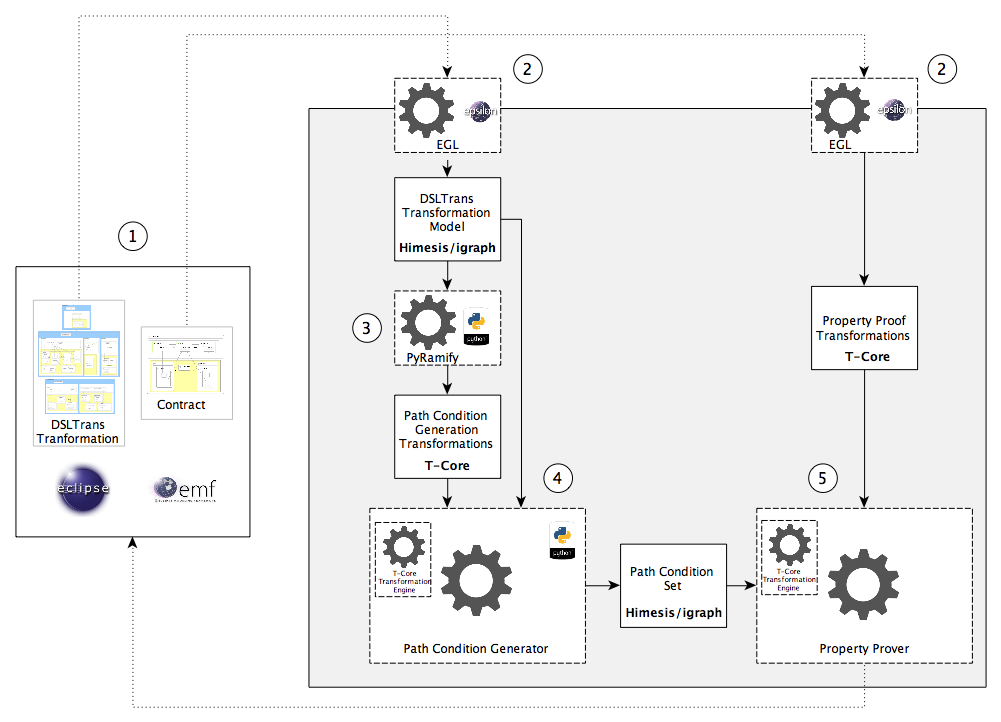
\includegraphics[width=0.8\textwidth]{figures/syvolt_prover/tooling_arch}
\caption{The architecture of the SyVOLT tool}
\label{fig:arch}
\end{figure*}


Figure~\ref{fig:arch} shows the
architecture of the SyVOLT tool. Two essential blocks are depicted: the
graphical front-end and the proof engine back-end. While the front-end
is responsible for the interaction with SyVOLT's user, the back-end implements
the algorithm for running the proofs of the contracts.

Note that two kinds of
communication occur between SyVOLT's front-end and back-end: in the
left-to-right direction, a number of artifacts (models and model
transformations) are syntesized from the graphical representations of the
DSLTrans transformations and of the SyVOLT contracts, and passed to the
back-end. In the reverse direction, the proof result and counter-examples, if
any, are passed from the proof engine back-end to the front-end.


\subsubsection{Generation of Transformation and Contracts}

As explained above, there are a number of ways to generate transformations and contract for the proving process. This section will describe the technologies behind these front-ends.

\paragraph{Atom3}

\textbf{AToM$^3$}~\cite{atom3:2002}: AToM$^3$ is a
  meta-editor\markus{What is a meta editor? Never heard this before.} for
  model-driven development.
  It has been developed at the MSDL\markus{?} and is used for constructing,
  models, metamodels and model transformation rules, and for automatically 
  synthesising modeling environments\markus{editors, right?}.
  AToM$^3$ has been extensively used to support the construction and
  visualisation of models and model transformation rules required by the proof
  engine during the initial stages of the construction of SyVOLT. 
  Many of these artifacts were built during the construction
  of SyVOLT explicitely to develop and test the proof algorithm in a
  controlled environment. In the finished SyVOLT all these artifacts are automatically
  generated from their graphical representations in the Eclipse front-end.\\
  
\paragraph{Eclipse Plugin}

 \textbf{EMF} (Eclipse Modelling Framework)~\cite{emfTool}: SyVOLT makes
  use of EMF's Ecore format for the
  XMI~\footnote{\url{http://www.omg.org/spec/XMI/}} representation of DSLTrans
  transformations and SyVOLT's contracts within the Eclipse editors\markus{How
  is XMI relevant here? Don't see that.}.
  Note that EMF is only used in the Eclipse front-end, and that Ecore models are converted
  into the Himesis format for the contract prover engine to compute the
  proofs\markus{Why?}.\\
  
  
  Eclipse is a popular development environment\markus{More
  importantly, it is a platform for tool integration, in particular, for
  model-based tools. This makes it really relevant for SyVOLT.} and model
  transformation tools such as ATL~\cite{atlTool}, DSLTrans~\cite{Barroca2011} and
  EGL~\cite{eglTool} are integrated with the Eclipse Modeling Framework
  (EMF)~\cite{emfTool}.
  
  To take advantage of this ecosystem, SyVOLT integrates with EMF\markus{Also
  say something about Ecore?}.
  In EMF, models can be represented in a multitude of syntaxes, from graphical
  to textual, and this makes the interaction with SyVolt easier since the modeler
  can use the model editor that is most convenient. Internally, SyVOLT uses 
  the Himesis format~\cite{Provost2006} to represent models.
  
  The SyVolt contract editor is realized by a set of Eclipse plugins.
  The runtime architecture of this editor is the typical architecture of a
  Graphical Modeling Framework (GMF)
  \footnote{\url{http://www.eclipse.org/modeling/gmp/}} editor.
  What is important is how this editor was developed.
  
  As mentioned in Section~\ref{sec:mdd_gui}\markus{Not sure I have read it
  there.}, we used Eugenia[CITE] to quickly develop the SyVolt contract editor
  shown in Figure~\ref{fig:eclipse_frontend}.
  \markus{Don't take this personal, but: one can see tha the editor is
  automatically generated and didn't get a lot of love, actually. I would
  downplay the editor and say it is a useful and workable prototype, but probably
  requires more love to make it really user friendly!}
  
  \markus{Reading this, I agree with Levi's comment that there is too much about
  how it was developed. THis is not a tutorial on how to build graphical editors.
  I suggest to remove.} Eugenia consists of a set of annotations that are attached
  to the metamodel of SyVOLT contracts. An annotation can, for instance, specify
  that an atomic contract will be drawn as a rounded rectangle, with a specific
  color and a label that is equal to the name attribute of the contract.
  The annotations are not very expressive but they contain the essential
  information to generate a set of GMF models that, ultimately, describe a basic
  usable graphical editor.
  
  Each generated GMF model is concerned with one aspect of the editor and can be
  further customized to our needs. GMF models are much more expressive than the
  Eugenia annotations.
  For instance, the generated GMF tooling model prescribes the kind of tools that
  will be available in the toolbox (shown in the right of
  Figure~\ref{fig:eclipse_frontend}), their icons, labels, etc\ldots
  
  From the set of GMF models, a set of eclipse plugins are synthesized.
  These make up SyVolt graphical editor\footnote{A fixed structure textual editor
  is also provided but this editor lacks several usability improvements and,
  hence, is not appropriate to model SyVolt contracts.}.
  
  The original DSLTrans transformation is manipulated using the DSLTrans editor
  and is serialized in XMI format. Similarly, SyVOLT contracts are manipulated with the SyVolt graphical
  editor and serialized in XMI format.
  
  
\subsubsection{Generation of Proving Artifacts}

From the transformation and contracts, we require a particular textual format to be generated.

This format is \textbf{Himesis}~\cite{Provost2006}: Himesis is a typed graph representation
  format, built upon the open-source igraph~\cite{igraphTool} library. 
Himesis is used for several reasons: independence\markus{of?}, efficiency and
tool support.
Independence\markus{of?} is ensured because Himesis is very expressive and also
very simple, which means it will not change for the foreseeable
future\markus{That's not INDEPENDENCE! How about stability? REliability? Reads
weak.}.
In \cite{Syriani2010b}, it is reported empirically\markus{what does ``reported
empirically'' mean?} that Himesis is a good format to perform typical graph
manipulation operations and it is seamlessly supported by T-Core\markus{What's
that? WHy is this a good thing for Himesis?}.
  Himesis is used pervasively within SyVOLT to represent models of 
  DSLTrans rules and of SyVOLT contracts, as well as all the model
  transformation rules required by the proof algorithm.


\paragraph{Atom3}

From Atom3, the Himesis files were directly written using model-to-text code written within the Atom3 code.

\paragraph{Eclipse Plugin}

\textbf{EGL} (Epsilon Generation Language)~\cite{eglTool}: Converting
  Ecore models into Himesis models is achieved using EGL, a language from the
  Epsilon family. Besides easy integration with Eclipse and native support of
  the expressive
Epsilon Object Language (EOL~\cite{Kolovos}), EGL also provides tasks for the
Ant~\footnote{\url{http://ant.apache.org}} build tool, which was used to
orchestrate the multiple tools in the proving process.

The translation of DSLTrans transformations and SyVOLT contracts into Himesis
models and model transformation rules was achieved using the Epsilon Generation
Language (EGL~\cite{Rose2008}). More specifically, two EGL model-to-text model
transformations were used: one to generate the Himesis models\markus{How is a
Himesis more represented? YOu say you use a text generator, so this suggests
it's text?} representing of a DSLTrans transformation (marked (a) is
Figure~\ref{fig:arch}); another one to generate the T-Core model transformation
rules necessary to prove SyVOLT contracts (marked (b) is Figure~\ref{fig:arch}).

These model-to-text transformations are used to parse the Ecore models of a
DSLTrans model transformation under analysis and of the contracts to be proved.
From these Ecore models, the EGL transformations produce a number of Python
files containing classes that inherit from the Himesis library and that
represent models and T-Core transformation rules. These classes are loaded from
disk by the Python interpreter and become models and model transformations in
memory once they are instantiated by the proof engine back-end.


\paragraph{MPS}

To be completed...

\subsubsection{Additional Generation of Model Transformations for Proof
Construction: The PyRamify Script (3)}

Additional model transformations, other than the ones described in
Section~\ref{sec:gen_models_mt}, need to be generated for the property proof
algorithm to execute. These are the \emph{path condition generation} T-Core
model transformation\markus{``path condition generation T-Core model
transformations'' is too long!} (marked (c) is Figure~\ref{fig:arch}) that are
needed to perform the model manipulations for building a set of symbolic
executions given a DSLTrans model transformation. These model transformation
blocks\markus{blocks?} allow combining the rules of a DSLTrans model
transformation into a set of \emph{path conditions}, as per the algorithm
described in~\cite{Lucio2014}. Note that the path condition generation T-Core
transformations are fully generated from the set of rules of the DSLTrans
transformation being verified.
\markus{THis paragraph is really hard to understand (conceptually and
syntactically)!}

This additional model transformation generation step is achieved by the PyRamify
component. PyRamify is a Python script\markus{program instead of script?} that
takes as input Himesis graphs representing the rules in the transformation.
Then, through the RAMification procedure~\ref{KuhneMSVW09}, T-Core matchers and
rewriters for each rule are produced. Very briefly, while matchers allow the
contract prover to determine how rules might execute over a path condition being
built, rewriters properly combine the right-hand side of a DSLTrans rule with
that same path condition whenever necessary.\markus{I have absolutely zero idea
what you wanted to tell me here :-)}

% PyRamify is also responsible for producing additional T-Core model
% transformations used for analysing how the DSLTrans rules in a transformation
% depend on each other. Explain this further??



\subsubsection{Path Condition Generation (4)}

Once the required artifacts\markus{which?} have been produced, the prover moves
on to the path condition generation step. Each path condition will represent an
(infinite) set of concrete executions of the transformation, where each concrete
execution is an input/ouput pair. Path condition generation is operationally
achieved by executing, following the ordering of the rules in the DSLTrans
tranformation being analysed, the path condition generation transformations
(marked (c) is Figure~\ref{fig:arch}) generated by the \emph{PyRamify}
component\markus{This sentence is convoluted. Use several.}.

  \textbf{T-Core}~\cite{Syriani2010a}: T-Core is a collection of model transformation
  primitives developed at the MSDL, allowing fine-grained manipulation of
  models. It was initially built as a means to rapidly build
  high-level model transformation languages. T-Core has been used to
  successfully deconstruct and reconstruct several mainstream model transformation
  languages~\cite{}. The main operations of T-Core are model \emph{matching},
  model \emph{rewriting} and \emph{iterating} through a set of match sites in a model.
  The level of control in model manipulation, together with T-Core's speed and
  scalability when treating large models, suited our needs when
  implementing the property proof algorithm described in~\cite{Lucio2014}. Note that because
  T-Core is also an explicitly modeled model transformation language, a T-Core
  model transformation rule is also a (Himesis) model\markus{So T-Core is
  explicitly modeled in Himesis?}.\\



The path condition generation algorithm starts from the empty path condition,
representing the case where no rules in the transformation have executed. Then,
as each T-Core transformation in the path condition generation
transformations\markus{Can we omit this word? Can't we just call it the ``path
condition generator'' and say only once that it is actually a bunch of
transformations? THe word is just too long.} set is executed, each rule in the
DSLTrans model transformation under analysis is combined with the path
conditions generated thus far. As each rule is considered, the set of path
conditions will grow to represent all allowed rule combinations.

As the execution of a rule in a DSLTrans transformation may depend on the
previous execution of other rules, such dependencies are verified by the path
condition generation transformations in order to exclude impossible rule
combinations.\markus{I notice myself skipping stuff here. Too many technical
terms. VERY hard to understand.}

% The final set of path conditions produced by the algorithm will then abstract
% the infinite set of all concrete transformation executions. This is further
% described in~\cite{Lucio2014}, along with a formal discussion of the validity
% and completeness of this work.

Note that path condition generation is a complex task, difficult to fully model
as a single model transformation\markus{Why not model it as a sequence of
simpler transformations?}.
As such, the algorithm in this component has been implemented as a Python script
that is responsible for scheduling all the path condition generation
transformations in the right order\markus{Aha. You should say that you've
modularized it into many}.

This programmatic level of granularity of manipulation has allowed us to build
many optimizations to speed up the path condition generation process. Examples
of such optimizations are the caching of expensive match operations, or the
parallelization of the path condition generation algorithm.
 
\subsubsection{Contract Proof (5)}

Once the path conditions are generated, the proof that each contract holds or
does not hold can then be built. The \emph{contract proof} component requires
two inputs: the \emph{path conditions set} built by the path condition generator
(marked (d) is Figure~\ref{fig:arch}) and the \emph{property proof T-Core
transformations} (marked (b) is Figure~\ref{fig:arch}).

Pre-/postcondition contracts form an implication, which needs to be checked for
each path condition provided as input to the contract proof component. For a
contract to hold on a DSLTrans model transformation, the contract's implication
should hold for every path condition generated for that model transformation.
Checking if the implication between a contract's pre- and postcondition holds on
a path condition is achieved by attempting to find for each submodel of the path
condition that is isomorphic to the precondition's model, a submodel of the path
condition that is isomorphic to the postcondition's model\markus{Understood. Can
the sentence be simplified?}.

The computations on the existence of these sugraphs isomorphisms is done by the
property proof T-Core transformations\markus{simpler: ``property prover''}. Note
that, in this case, the T-Core transformations are simply a set of matchers, or
queries, as no further editing of the path conditions is necessary during this
part of the proof\markus{I don't understand this ``editing'' business. Why
should any of this stuff be edited as the proof executes?}.

As in the path condition generation component described in
Section~\ref{sec:path_cond_gen}, the contract proof algorithm has also been
implemented as a Python script that schedules all the property proof T-Core
transformations appropriately. As before, using fine-grained programmatic
manipulations of the models and model transformations involved in the contract
proof algorithm has allowed us to implement optimization strategies during
contract proof. The main of these strategies is the skipping of path conditions
for which the contract is sure to hold without further analysis, given some
existing cached information about similar path conditions.

\subsection{Discussion}

This section provides a brief post-mortem of the development of our contract prover. In particular, we highlight that current tooling lacks support for building the complex model artifacts that we require.

Discussing limitations of model-driven technology here.


\subsubsection{Generation of Himesis}

Note that, while this approach of building models and model transformations as
textual files is sufficient for our needs, it is not ideal from the model-driven
development viewpoint. Building models as textual files forces us to deal to
the accidental complexity of Python code and of the Himesis format, making the
generation of these artifacts more difficult and error prone than it needs to
be. The issues encountered here expose one of the current important fragilities
of model-driven development: the difficulty of exchanging high-level data
between different modelling frameworks~\levi{cite benoit combemale here}.
\markus{Hmmmm. You can easily create an AST of Python and then M2M to this one,
and serialize. I would, again, not discuss this here. I'd just say that this
was the simplest thing to do, and since it's not the object of the tool, that's
what you did. That's it. Don't try to ``scientificate'' it.}

\subsubsection{Generation of Prover Transformations}

Currently, PyRamify is implemented as a Python script, as we were unable to
implement at the time automatic creation of higher-order artifacts (in our
case, T-Core transformations) from models in another modelling tool.
This was due to the mix of different modelling abstraction levels present in
SyVOLT and that led to a number of technical difficulties.

We have recently learned that, alternatively, \emph{path condition generation
transformations} could be built directly from the Ecore representation of
DSLTrans rules by using EGL technology -- as was done for the artifacts
described in Section~\ref{sec:gen_models_mt}. Nevertheless, a preferred solution
for us would be to use model transformation technology that that explicitely
allows building model transformations from simple models. To the best of our
knowledge, model transformation technology that allows moving between models of
a given order $n$ and an order $n+1$ is not yet available in the modelling
community.\markus{Isn't this part of a discussion of future work? As a reader,
I am really bored (annoyed??) by this level of detail here. I really don't
care.}
